\documentclass[a4paper, 12pt]{book}
\usepackage{graphicx}
\usepackage[french]{babel}
\usepackage[utf8]{inputenc}
\usepackage[T1]{fontenc}
\usepackage{multirow}
\usepackage{listings}
\usepackage{float}
\usepackage{url}
\usepackage[french]{algorithm}
\usepackage{style/myalgorithm}
\usepackage{amsmath,amsfonts,amssymb}
\newcommand{\fBm}{\emph{fBm}~}
\newcommand{\etal}{\emph{et al.}~}
\newcommand{\glAd}{\emph{GL4D}~}
\newcommand{\apiopengl}{API OpenGL\textsuperscript{\textregistered}~}
\newcommand{\opengl}{OpenGL\textsuperscript{\textregistered}~}
\newcommand{\opengles}{OpenGL\textsuperscript{\textregistered}ES~}
\newcommand{\clang}{langage \texttt{C}}
\newcommand{\codesource}{\textsc{Code source}~}
\floatstyle{ruled}
\newfloat{programslist}{htbp}{locs}
\newcommand{\listofprograms}{\listof{programslist}{Liste des codes source}}
\newcounter{program}[subsection]
\renewcommand{\theprogram}{\arabic{chapter}.\arabic{program}}

\newenvironment{program}[1]{
  \if\relax\detokenize{#1}\relax
  \gdef\mycaption{\relax}
  \else
  \gdef\mycaption{#1}
  \fi
  \refstepcounter{program}
  \addcontentsline{locs}{section}{#1}
  \footnotesize
}{
  \begin{description}
    \item[\codesource \theprogram]--~\mycaption
  \end{description}
}

\begin{document}
\begin{titlepage}
  \begin{center}
    \begin{tabular*}{\textwidth}{l@{\extracolsep{\fill}}r}
      
\includegraphics[height=1.5cm]{images/logo_liv.png}&
      
\includegraphics[height=1.5cm]{images/oaccueil.png}
    \end{tabular*}
    \small 
    \rule{\textwidth}{.5pt}~\\
    \large 
    \textsc{Université Paris 8 - Vincennes à Saint-Denis}\vspace{0.5cm}\\
    \textbf{Licence informatique \& vidéoludisme}\vspace{3.0cm}\\
    \Large
    \textbf{Modèle pour projet tuteuré ou rapport de stage}\vspace{1.5cm}\\
    \large
    \textbf{Farès \textsc{Belhadj}}\vspace{1.5cm}\\
    Date de soutenance : le JJ/MM/AAAA\vspace{1.75cm}\\
  \end{center}\vspace{1.5cm}~\\
  \begin{tabular}{ll}
    \hspace{-0.45cm}Organisme d'accueil~:~&~XXXXXXX (si stage)\\
    \hspace{-0.45cm}Tuteur -- Organisme d'accueil~:~&~Prénom \textsc{Nom} (si stage)\\
    \hspace{-0.45cm}Tuteur -- Université~:~&~Prénom \textsc{Nom}\\
  \end{tabular}
\end{titlepage}
\frontmatter
\chapter*{Résumé}
\markboth{\sc Résumé}{}
\addcontentsline{toc}{chapter}{Résumé} 

Le présent document sert aussi bien de \emph{template} que de guide
des bonnes pratiques de rédaction d'un mémoire de stage ou d'un
mémoire de projet tuteuré. Il est à destination des étudiants en
\emph{Licence informatique \& vidéoludisme} de l'Université
Paris 8 ainsi qu'à toute personne trouvant un intérêt à
l'utiliser. \`A ce titre il est distribué selon la licence GPL
(\emph{GNU Public Licence}) et vous pouvez en télécharger les sources
à l'adresse~: \url{https://expreg.org/amsi/C/LIV/}.\\


Attention, le résumé est la partie à rédiger en dernier. Dans un
premier temps, vous devez, en deux phrases maximum, décrire le travail
réalisé et détaillé dans ce mémoire. \`A la suite de ces deux phrases,
allez un peu plus en profondeur et tentez de suivre un raisonnement
vous emmenant à votre conclusion. Tout ceci doit aboutir à un
paragraphe d'une demi-page permettant d'avoir une idée claire du
travail effectué et des contributions. Enfin, la deuxième partie du
résumé doit suivre le déroulement du mémoire et donner en une ou deux
phrases le contenu de chaque chapitre : \guillemotleft{}~Dans le
premier chapitre, nous\footnote{Vous remarquerez l'usage du
  \emph{nous} ; cette forme est \textbf{obligatoire} dans la rédaction
  d'un mémoire. Aussi, bannir l'usage du \emph{on} car comme dit
  l'expression \guillemotleft{}~On est un c...~\guillemotright. Dernier
  point, ceci est une \emph{footnote} (note de bas de page) et, même
  si c'est présentement le cas, nous vous prions de ne pas insérer ce
  type de notes dans le résumé.} ... Puis, nous détaillons ... dans le
chapitre suivant ... Enfin, en conclusion nous ...~\guillemotright
\chapter*{Remerciements}
\markboth{\sc Remerciements}{}
\addcontentsline{toc}{chapter}{Remerciements} La page des
remerciements n'est pas obligatoire. Elle reste votre seul vrai espace
de liberté complet. Il existe néanmoins une codification classique des
remerciements consistant à remercier les personnes que vous citez de
la relation la plus strictement professionnelle et hiérarchique à la
relation la plus personnelle.
%% Table des matières
\tableofcontents
%% La liste des figure est optionnelle (si votre rapport manque de
%% contenu ajouter ce type de pages sera perçu négativement)
\listoffigures
%% La liste des programmes est optionnelle (si votre rapport manque de
%% contenu ajouter ce type de pages sera perçu négativement)
\listofprograms
\mainmatter
\chapter*{Introduction}
\markboth{\sc Introduction}{}
\addcontentsline{toc}{chapter}{Introduction}
L'introduction peut être vue comme une version détaillée du résumé
mais peut traiter de choses qui n'ont pas été citées dans ce
dernier. Elle doit être écrite juste avant d'écrire le résumé
(cf. section \ref{sec-ordre-redaction})\footnote{Jetez un \oe{}il au
  code \LaTeX{} du présent document pour voir comment sont réalisées
  les références dynamiques. Commandes utilisées~:
  \texttt{\textbackslash{}ref} et
  \texttt{\textbackslash{}label}.}.\\~\\ Dans une introduction~:
\begin{itemize}
\item \textbf{Vous devez} bien poser le contexte de votre mémoire,
  ceci comprend~: la mission et son environnement ; un bref descriptif
  de la (ou des) problématique(s) et les outils et méthodes imposées
  ou choisies\footnote{\`A chaque fois que vous proposez plusieurs
    \emph{items} dans une phrase, arrangez-vous pour en avoir au
    minimum trois (n'en proposez pas trop non plus). Ceci donne un bon
    rythme à votre texte~: un, deux et trois. \emph{Thanks to \sc
      PG}.} ;
\item \textbf{Vous devez} résumer les résultats ou solutions apportées
  et éventuellement faire un mini-bilan par rapport à l'existant ;
\item Lors de la rédaction d'un mémoire de stage, \textbf{vous pouvez}
  brievement présenter la structure d'accueil au moment où vous posez
  le contexte du mémoire mais ne soyez pas trop long surtout si vous
  réservez une section de chapitre à cela\footnote{Il n'est pas
    recommandé de réserver un chapitre entier à la seule présentation
    de l'organisme d'accueil, vous pouvez par exemple insérer la
    présentation de l'organisme dans un chapitre détaillant le contexte
    et la problématique du stage.} ;
\item \textbf{Vous pouvez} insérer une section \emph{\'Etat de l'Art}
  dans l'introduction si ce dernier n'est pas assez conséquent (par
  exemple lors d'un stage dans l'industrie) ou que le mémoire n'est
  pas lui-même un \emph{\'Etat de l'Art}. Pour un projet tuteuré ou un
  mémoire de stage \emph{Recherche}, un chapitre \emph{\'Etat de l'Art}
  est fortement conseillé.
\end{itemize}
\chapter{Les chapitres}
Ceci est un \emph{chapeau de chapitre}. Il a pour fonction de résumer
le contenu d'un chapitre et il est obligatoire. Il faut toujours le
ridiger une fois le contenu propre au chapitre terminé.\\


Dans ce chapitre, nous commençons par donner la composition du
mémoire, la forme littéraire à employer, nous énumérons l'odre de
rédation des différentes composantes du mémoire puis nous ...
\section{Structuration du document}
Un mémoire (de classe \texttt{book} en \LaTeX) est composé d'une page
de garde\footnote{Nous allons vérifier que vous avez attentivement lu
  l'ensemble du document. Sur la page de garde, veuillez supprimer
  l'un des deux logos de formation en gardant celui vous
  concernant. Il ne faut pas oublier de supprimer le
  \guillemotleft{}~--~ou~--~\guillemotright{} présent entre les deux
  logos. Aussi, veillez à mettre \textbf{vos} \guillemotleft{}~{Prénom
    \sc Nom}~\guillemotright{} en lieu et place de ceux de l'auteur du
  présent document.}, d'un résumé, de chapitres, de listes et
éventuellement d'annexes. Certains chapitres sont numérotés, d'autres
non (Remerciements et Introduction). Les chapitres peuvent être
composés de sections et ces dernières de sous-sections ... (essayez de
ne pas dépasser la profondeur sous-sous-section). \`A chaque fois que
vous estimez nécessaire de descendre d'un niveau (ex. du chapitre vers
des sections), il faut respecter la règle suivante : rédiger un
\emph{chapeau} et avoir au minimum deux instances du niveau
inférieur. Par exemple, pour un chapitre, si vous souhaitez créer une
section alors vous devez obligatoirement en avoir au minimum deux et
rédiger un \emph{chapeau de chapitre} qui vient se placer avant la
première section.
\section{Forme littéraire du document}
Votre rapport de projet tuteuré ou mémoire de stage de fin d'études
prend la forme d'un exposé scientifique traitant d'une ou plusieurs
problématiques dans un contexte donné, apportant des solutions
partielles, des évaluations de ces solutions et des conclusions
ouvertes sur des perspectives. Ce document expose des faits regroupés
par thème ou problématique et ne doit pas prendre la forme d'un récit
chronologique. Par ailleurs, l'usage du pronom \emph{Nous} y est
obligatoire et le temps \emph{présent} est de mise\footnote{Des
  exceptions sont néanmoins possibles mais il est préférable d'en
  limiter le nombre. Ainsi, nous pourrons par exemple dire :
  \guillemotleft{}~Ces travaux ont donné lieu à une publication
  scientifique dans la revue ...~\guillemotright{} ou
  \guillemotleft{}~L'algorithme de planification de trajectoire a été
  implémenté avec succès sur la flotte de robots
  ...~\guillemotright.}.
\section{Dans quel ordre rédiger son mémoire\label{sec-ordre-redaction}}
\noindent{}Nous proposons, ci-après, une liste de règles à suivre pour
bien réussir la rédaction de son mémoire~:
\begin{description}
\item[Le plan~:] toujours commencer par l'élaboration d'un plan. Il est
  utile que le plan soit soumis au tuteur pour validation. Dans une
  moindre mesure, le plan définitif peut dévier de la version initiale
  ;
\item[L'état de l'art~:] s'il y a lieu, comme section de
  l'Introduction ou chapitre à part entière, il est là pour justifier
  votre approche et les raisons de vos choix. Cette partie pouvant
  être assez difficile à rédiger, vous pouvez faire des aller-retours
  avec le point suivant en cas de blocage rédactionnel (\emph{ie.}
  l'angoisse de la page blanche) ;
\item[Les chapitres \guillemotleft{}~techniques~\guillemotright{}~:]
  une fois le plan approximativement déterminé, vous pouvez commencer
  à rédiger les parties les plus techniques (les schémas techniques,
  les implémentations, les tests, ...). Elles sont généralement plus
  faciles à écrire car elles décrivent des faits avérés et vous
  n'aurez pas besoin de beaucoup d'argumentaire pour les
  justifier. Ceci ne vous dispense pas de la partie argumentaire --
  \emph{pour quelles raisons ces choix ont été faits} -- qui peut
  arriver plus tard dans le processus rédactionnel. La justification
  des choix effectués peut-être faite au niveau de chaque chapitre ou
  au niveau de l'état de l'art et de l'Introduction ;
\item[Les chapeaux de chapitres et conclusions de chapitres~:] une
  fois le c\oe{}ur d'un chapitre écrit, vous pouvez rédiger son
  chapeau qui est obligatoire à terme, et, éventuellement, vous pouvez
  ajouter une conclusion de chapitre. Ces deux parties décrivent
  brievement le contenu du chapitre mais pas de la même manière. L'un
  (le chapeau) introduit et déroule le contenu dans son contexte et
  éventuellement ses justifications, l'autre (la conclusion du
  chapitre) revient sur le contenu en s'appuyant sur les résultats et
  les conlusions à en tirer et peut même faire la liaison avec le
  chapitre suivant ;
\item[L'Introduction générale~:] à écrire une fois tous les chapitres
  rédigés sans nécessairement avoir les chapeaux de chapitres et les
  conclusions de chapitres. Pour le contenu de l'introduction, voir le
  chapitre Introduction du présent document ;
\item[La Conclusion et Perspectives~:] à ce stade il ne vous reste
  plus que la conclusion générale et le résumé. Voir le chapitre
  \ref{chap-conclusion} pour le contenu de la conclusion ;
\item[Le résumé~:] est la partie à écrire en dernier, elle doit être
  rédigée selon les recommandations données dans le Résumé du présent
  document.
\end{description}

Une fois tous les points terminés, n'oubliez pas de faire une passe de
\emph{ispell}\footnote{Le correcteur orthographique est
  obligatoire. Si un document comporte trop de fautes d'orthographe,
  le lecteur se focalise sur celles-ci et n'arrive plus à évaluer le
  fond.}, de relire votre document, de le faire relire par des amis ou
des proches et enfin de le soumettre à votre tuteur.
\section{Insertion d'éléments dans le document}
Cette section traite de l'insertion d'éléments externes dans le
mémoire. C'est une partie technique dont vous devez consulter le code
source pour acquérir les notions \LaTeX{} liées aux types d'objets
insérés.
\begin{figure}[htbp]
  \centering
  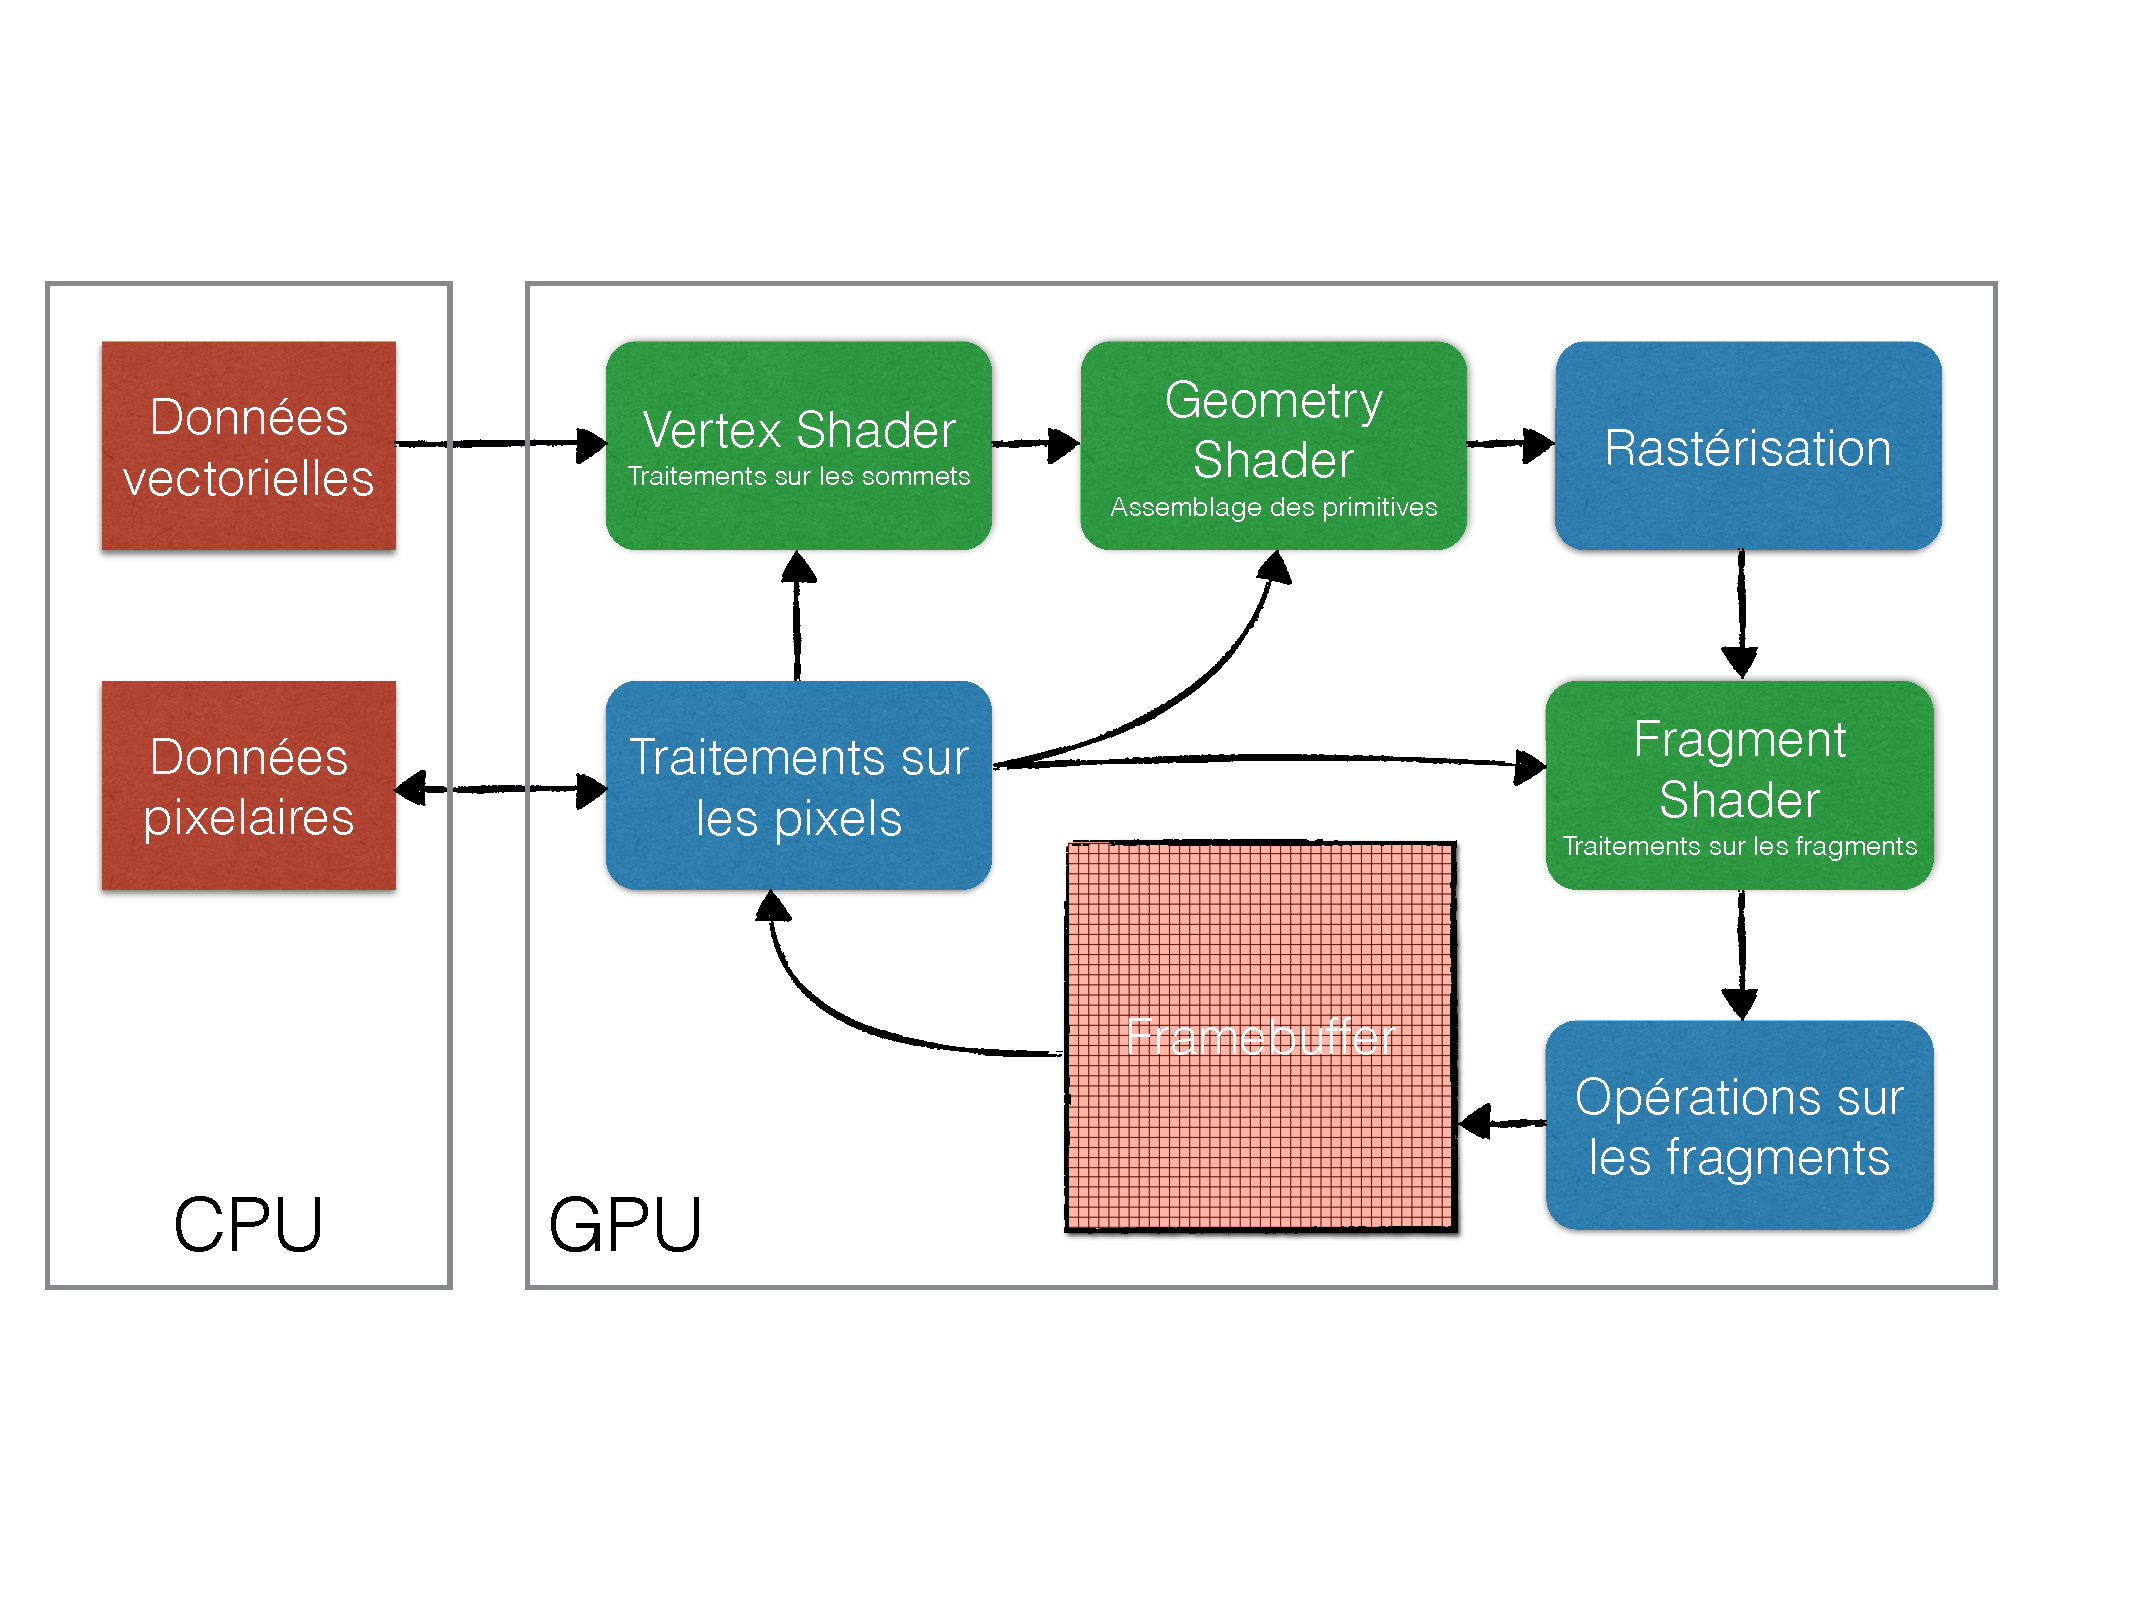
\includegraphics[width=0.5\linewidth]{fig/pipeline.pdf}
  \caption{Schéma vectoriel inclus depuis un fichier \texttt{pdf}. Ne
    pas hésiter à faire de la redite au niveau des titres de
    figures, leur lecture doit se suffir à elle-même.\label{fig-vect}}
\end{figure}


\subsection{Les images et figures}
Réaliser ses images et figures c'est, comme dit l'expression,
\emph{manger son pain blanc}\footnote{J'ai découvert l'usage de
  l'expression \emph{manger son pain blanc} par le biais de mon ami et
  collègue Vincent Boyer qui, entre autres, aime toujours à expliquer
  les concepts de façon imagée. Par ailleurs, je le remercie pour ses
  conseils et relectures du présent document.}. Ceci est pris dans le
sens où cette tâche est assez aisée comparée au fait de rédiger des
parties complexes du mémoire comme les argumentaires. De plus, le fait
d'insérer des figures augmente rapidement le nombre de pages du
mémoire. Ce qui implique aussi l'obligation de ne pas en abuser ;
chaque figure doit avoir une réelle justification à sa présence dans
le document. Un dernier conseil, ne mangez pas tout votre pain blanc
d'un coup, laissez-en pour les périodes d'angoisses de pages blanches.


Trève de discours, nous pouvons voir, en Figure \ref{fig-vect}, un
exemple de schéma vectoriel inclus depuis un fichier
\texttt{pdf}. 

Aussi, en Figure \ref{fig-bmp}, nous présentons une
image importées depuis un fichier \texttt{png}. Toute figure présente
dans le document doit être citée au moins une fois dans le
texte. 

\begin{figure}[htbp]
  \centering
  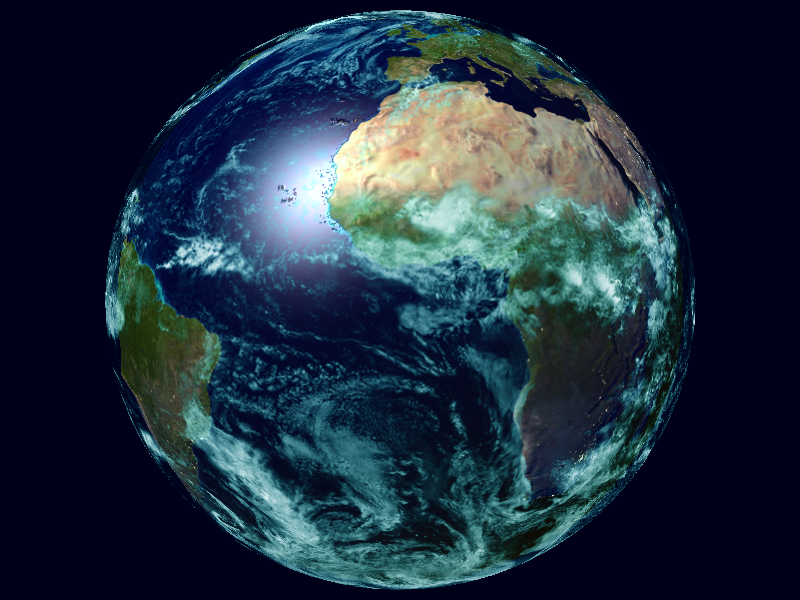
\includegraphics[width=0.5\linewidth]{images/earth_06_rendu_final.png}
  \caption{Image bitmap importée depuis un fichier \texttt{png}. Ne
    pas hésiter à faire de la redite au niveau des titres de
    figures, leur lecture doit se suffir à elle-même.\label{fig-bmp}}
\end{figure}




Enfin, la Figure \ref{fig-tab}, est une composition des deux
précédentes et utilisant l'environnement \texttt{tabular}.

\begin{figure}[htbp]
  \centering
  \begin{tabular}{cc}
    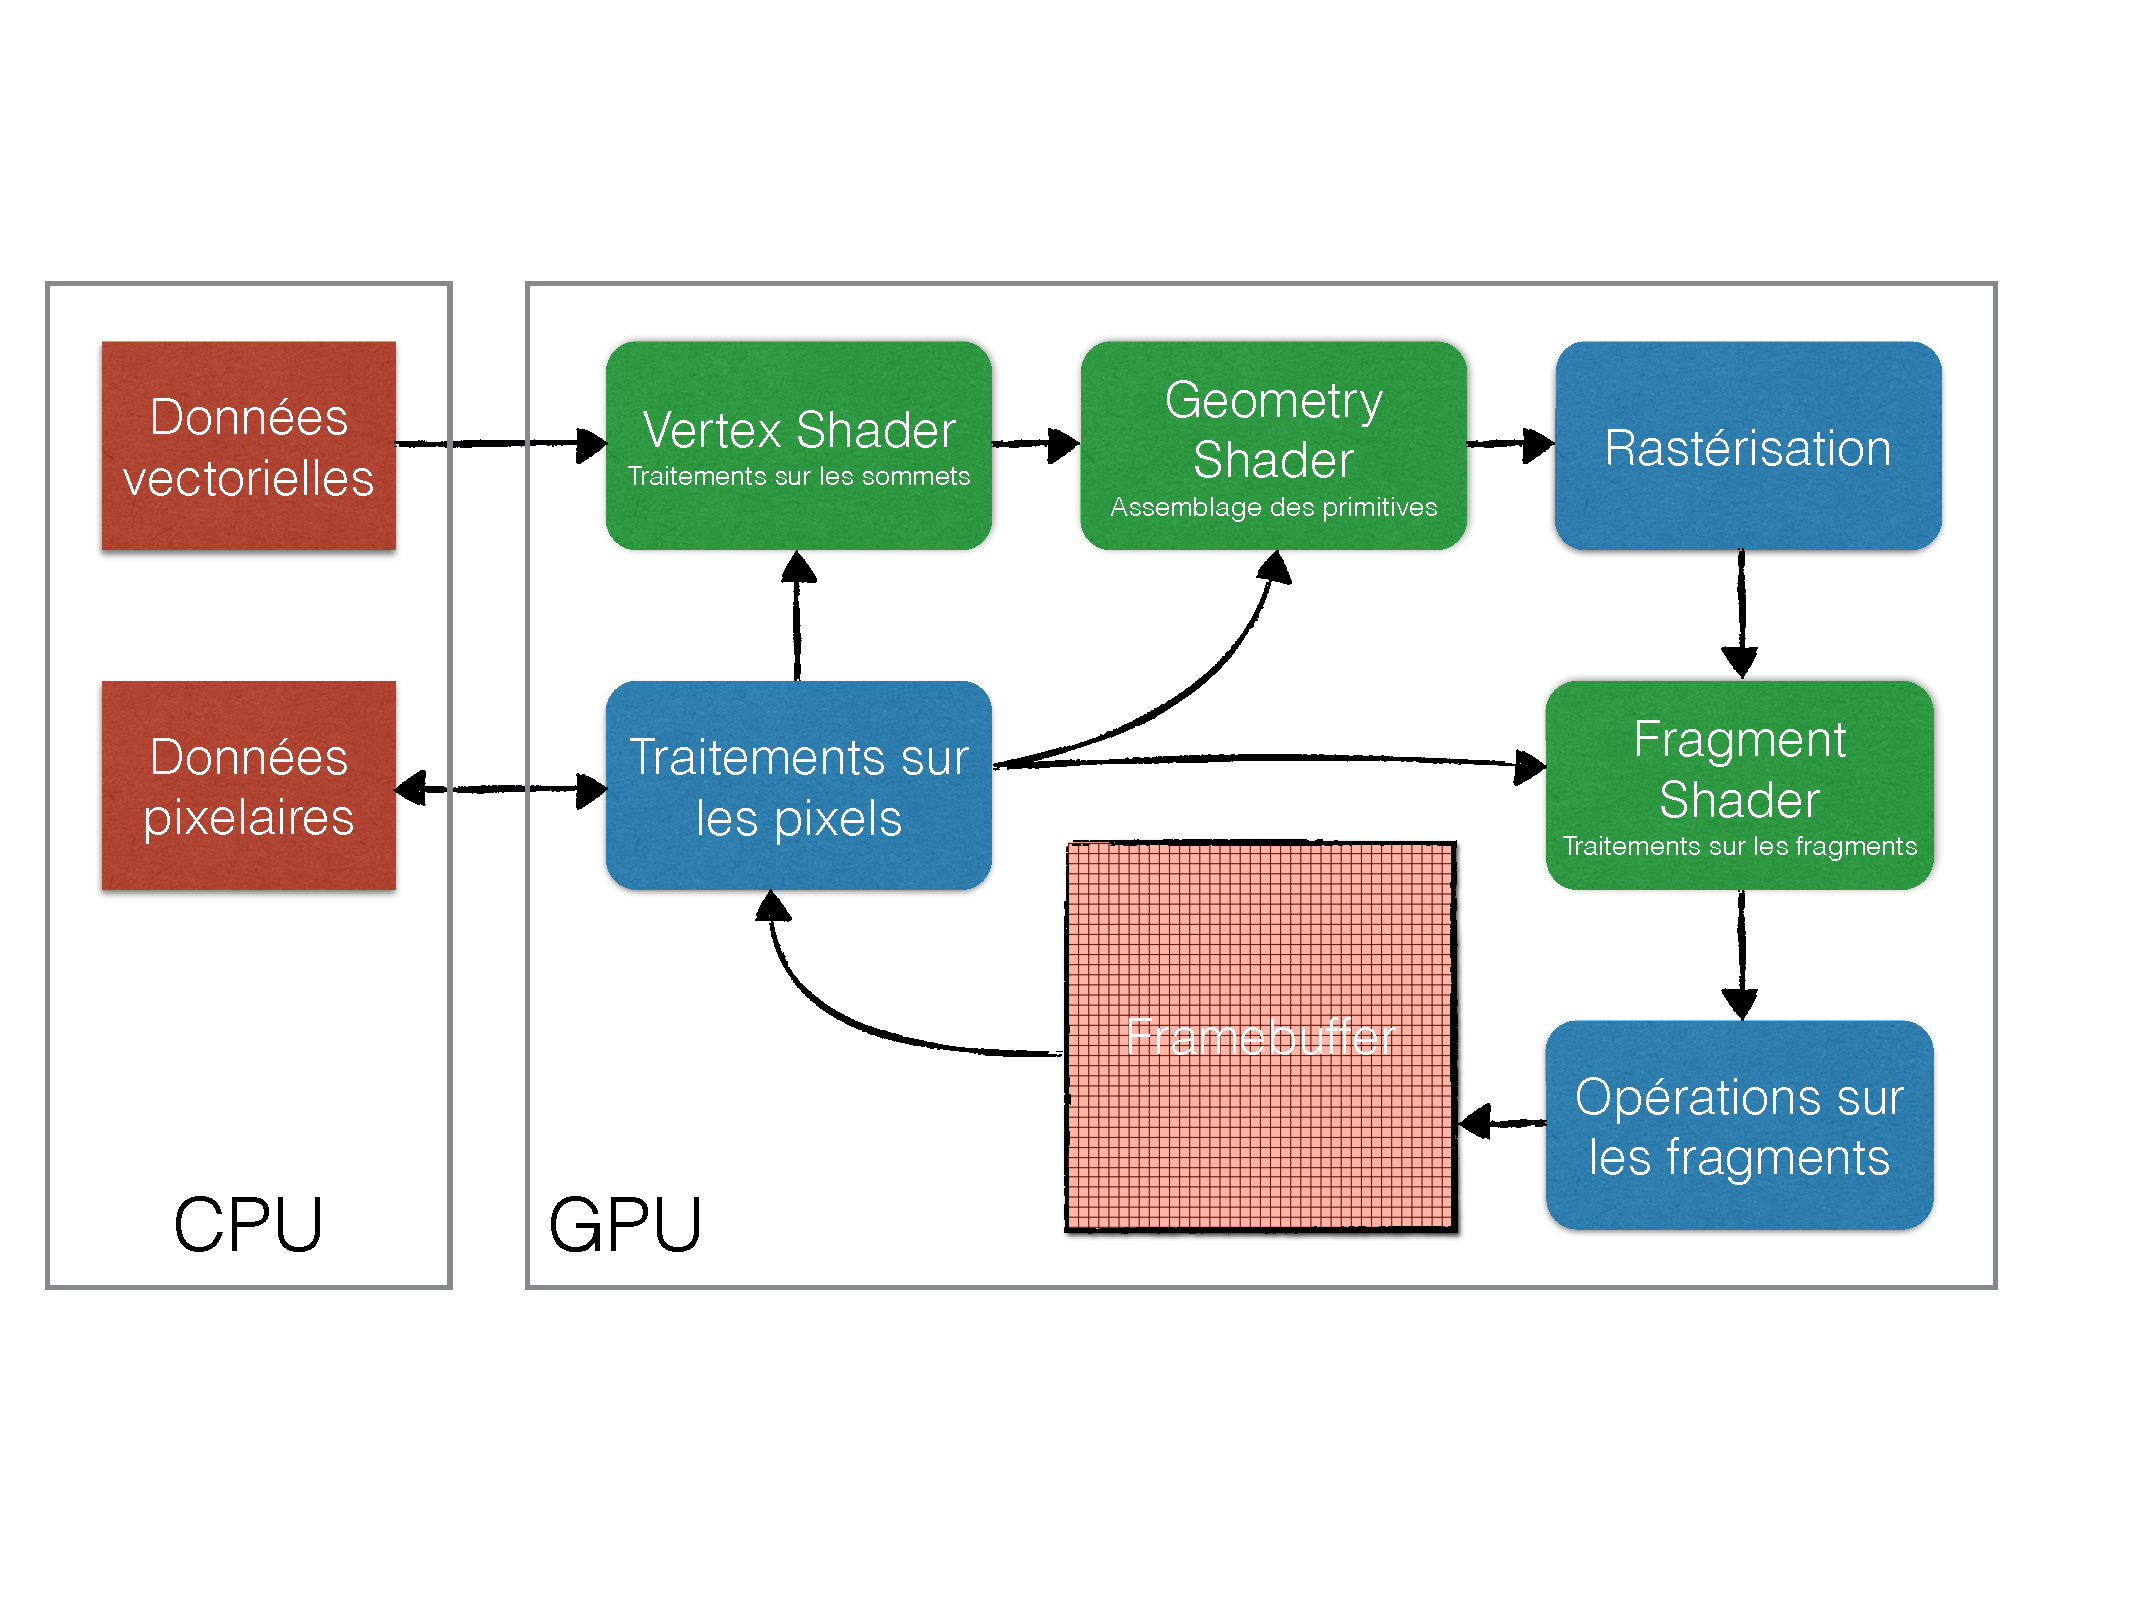
\includegraphics[height=0.15\textheight]{fig/pipeline.pdf}&
    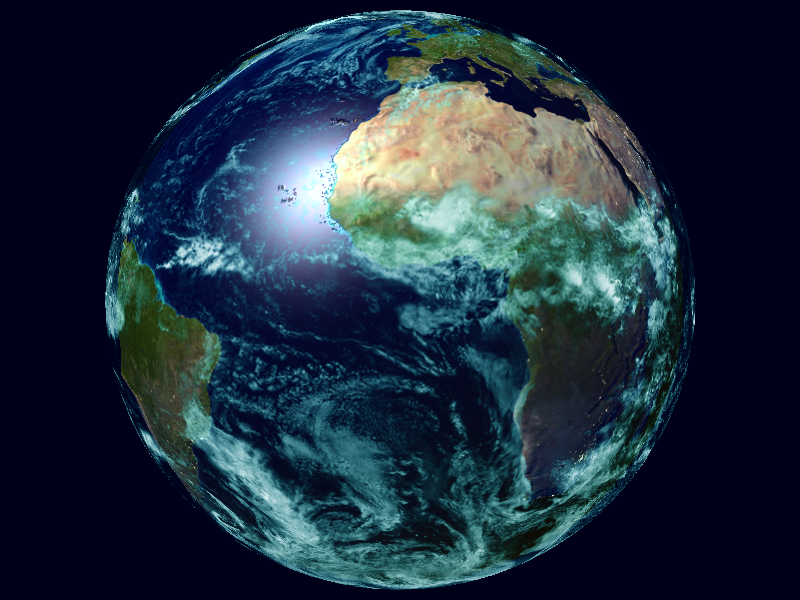
\includegraphics[height=0.15\textheight]{images/earth_06_rendu_final.png}\\
    (a)&(b)
  \end{tabular}
  \caption{Figure composée de deux images~: (a) une vectorielle ; (b) une bitmap.\label{fig-tab}}
\end{figure}

\subsection{Les formules mathématiques}
En \LaTeX, les formules mathématiques sont gérées dans l'environnement
mathématique. Il existe deux manières d'insérer des formules~:
\begin{itemize}
  \item Directement dans le texte entre deux symboles \texttt{\$}
    quand par exemple nous déclarons une variable $x$ et que nous
    définissons son intervalle telle que $x \in [0,1]$, ou bien $x \in
    \mathbb{R}$. Nous pouvons aussi lui donner une valeur telle que $x
    = \frac{1}{2}$ ou la déclarer comme une somme $x =
    \sum_{i=0}^{n-1}i$;
  \item Mais peut-être serait-il plus pratique de poser les formules
    en dehors du texte à l'aide des doubles \texttt{\$\$}~:
    
    $$ \forall i \in \mathbb{N}^{*}, \exists x \in ]0.5, 1[ \mbox{~tel que~} x = \sum_{i=1}^{n}\frac{1}{2^i} $$
        ou pour définir un système d'équations~:
        \begin{eqnarray}
        \left\{
        \begin{array}{lll}
          2\times{}x + y &= &1\\
          3\times{}x^2 - 2\times{}y &= &0
        \end{array}
        \right.
        \end{eqnarray}
\end{itemize}
\subsection{Les algorithmes}
Au même titre qu'une figure, un algorithme doit être cité dans le
texte. L'algorithme \ref{algo-bas-haut} calcule les positions
manquantes à un déplacement des milieux classique afin qu'il puisse
prendre en compte des contraintes quelconques.
\begin{algorithm}
  \begin{algorithmic}
    \footnotesize
    \REQUIRE Les éléments définis en début de section.
    \ENSURE le MNT $\mathcal{T}$ complété.
    \FORALL{$y\in\{0,1,2, ..., H - 1\}$}
    \FORALL{$x\in\{0,1,2, ..., L - 1\}$}
    \STATE \textbf{si} {$\mathcal{T}[y][x].e \ne inconnu$} \textbf{alors} \texttt{enfiler($\mathcal{FPA}$, ($x$,$y$))}
    \ENDFOR
    \ENDFOR
    \WHILE{($n\leftarrow $ \texttt{nb\_elts($\mathcal{FPA}$)}) $\ne 0$}
    \FORALL{$i\in\{1,2, ..., n\}$}
    \STATE $(e_x, e_y)\leftarrow $ \texttt{defiler($\mathcal{FPA}$)}
    \FORALL{$(p_x,p_y)\in$ \texttt{simu\_dm($L$, $H$, ($e_x$, $e_y$))}}
    \STATE \textbf{si} {$\mathcal{T}[p_y][p_x].e \ne inconnu$} \textbf{alors \textsc{Continuer}}
    \STATE $\mathcal{E}x[p_y][p_x].a \leftarrow \mathcal{E}x[p_y][p_y].a + \mathcal{T}[e_y][e_x].a$
    \STATE $\mathcal{E}x[p_y][p_x].n \leftarrow \mathcal{E}x[p_y][p_y].n + 1$
    \STATE $\mathcal{E}x[p_y][p_x].d \leftarrow \mathcal{E}x[p_y][p_y].d + \sqrt{(p_x - e_x)^2 + (p_y - e_y)^2}$
    \STATE \texttt{enfiler($\mathcal{FPA}$, ($p_x$,$p_y$))}
    \ENDFOR
    \ENDFOR
    \STATE $n\leftarrow $ \texttt{nb\_elts($\mathcal{FPA}$)}
    \FORALL{$i\in\{1,2, ..., n\}$}
    \STATE $(p_x, p_y)\leftarrow $ \texttt{elt\_file($\mathcal{FPA}$, $i$)}
    \STATE $\mathcal{T}[p_y][p_x].a \leftarrow \frac{\mathcal{E}x[p_y][p_x].a}{\mathcal{E}x[p_y][p_x].n} + \frac{\mathcal{E}x[p_y][p_x].d\times s}{\mathcal{E}x[p_y][p_x].n} \times X$
    \STATE $\mathcal{T}[p_y][p_x].e \leftarrow connu$
    \ENDFOR
    \ENDWHILE
    \STATE \texttt{dm($\mathcal{T}$, $s$, $t$, $\mathcal{H}$)}
  \end{algorithmic}
  \caption{Déplacement des milieux, l'approche bas-haut-bas.\label{algo-bas-haut}}
\end{algorithm}
\subsection{Le code source}
Toujours la même contrainte que précédemment, tout code source inclus
doit être cité dans le texte. Ainsi, le code source \ref{code-md} est
une inclusion de code en langage \texttt{C}. De manière générale, nous ne
recommandons pas l'inclusion de codes trop longs, contentez-vous des
portions les plus significatives si ces dernières ont un réel intérêt.\\

\begin{program}{Déplacement des milieux en une dimension\label{code-md}}
  \centering
  \fbox{\lstinputlisting[language=C]{sources/md.c}}
\end{program}

\section{La bibliographie et les citations}
La bibliographie est gérée par l'outil \texttt{BibTeX}, ce dernier
utilise un fichier externe pouvant contenir plusieurs entrées
bibliographiques (cf. fichier \texttt{memoire.bib}). Chaque entrée
devant être insérée à votre mémoire doit être citée dans le texte via
la commande
\texttt{\textbackslash{}cite\{reference\_de\_l\_entree\}}. Par
exemple~:
\guillemotleft{}~Prusinkiewicz~\cite{prusinkiewicz93moutainswithrivers}
décrit un modèle de génération d'un terrain fractal couplé avec une
génération de rivière, le tout en une seule passe~\guillemotright. Dans
le fichier bibliographique donné en exemple, vous trouverez plusieurs
formes d'entrées bibliographiques~: un livre~\cite{redbook}, un
chapitre d'ouvrage~\cite{texturing_and_modeling}, un article de
revue~\cite{musgrave89synthesis}, un article de
conférence~\cite{prusinkiewicz93moutainswithrivers}, une
thèse~\cite{boyer}, une url~\cite{srtm}, ... \'Eviter l'usages des
termes \emph{webographie} ou (pire\footnote{Au fait, je ne sais pas
  quelle est la pire (ceci est une mauvaise \emph{footnote}, car une
  \emph{footnote} doit se suffir à elle-même).}) \emph{netographie}
dans votre document.


Pour les citations, toute phrase provenant d'un autre document, ou
même traduite depuis un document rédigé dans une autre langue doit
être présentée entre guillemets (commandes \texttt{guillemotleft} et
\texttt{guillemotright}) et l'origine du texte doit être clairement
identifiée. A défaut, vous risquez d'être accusé de plagiat~:
\guillemotleft{}~Le plagiat est puni par la loi française et passible
de sanctions. En cas de détection de plagiat, la note de zéro peut
être attribuée à l’épreuve concernée et l’étudiant est renvoyé à la
seconde session ...~\guillemotright{} -- extrait du site de
l'INP-Toulouse -- Nous rajouterons que pour les soutenances de stage
et pour les projets tuteurés il n'y a pas de seconde session.
\chapter{Conclusion et Perspectives\label{chap-conclusion}}
Vous arrivez à la presque-fin de votre périple (oui il restera le
résumé à faire, rappelez-vous), la conclusion. Ici, il est attendu
d'avoir un bilan du travail réalisé\footnote{Ne pas utiliser de
  formules du type \guillemotleft{}~Ce stage a été très
  enrichissant~\guillemotright{} ou \guillemotleft{}~Ce projet m'a
  beaucoup apporté sur le plan professionnel ou
  personnel~\guillemotright{} car si le travail en question est
  important ou intéressant le mémoire doit naturellement le
  refléter.}. Ce dernier doit être consolidé par les réalisations et
les résultats obtenus. Il est utile de rappeler les améliorations
apportées en les replaçant brievement dans leur contexte. Aussi, il est
conseillé d'avoir un point de vue critique vis-à-vis de votre travail
et souligner les points pouvant être améliorés. Ceci s'enchainera
parfaitement avec les perspectives qui ouvrent la voie vers les
nouvelles réalisations possibles sur la base de vos travaux. Les
perspectives peuvent être données à court, moyen et long terme.



Par exemple, une conclusion à ce document peut être~:
\guillemotleft{}~Dans ce document, nous avons présenté un ensemble de
règles permettant d'écrire un mémoire de stage ou de projet
tuteuré. Ce document utilise un langage de formatage de texte nommé
\LaTeX. En perspectives, nous souhaitons que l'ensemble des étudiants
lisent attentivement et utilisent ce document. Enfin, nous pensons que
ce type d'exercie deviendra un standard pour chacun
d'entre-eux~\guillemotright.

\bibliographystyle{alpha}
\bibliography{memoire}
\end{document}
